\documentclass[10pt,twocolumn]{article}
\usepackage[letterpaper,margin=0.75in]{geometry}
\usepackage{amsmath,amssymb}
\usepackage{tikz}
\usetikzlibrary{arrows,arrows.meta,backgrounds,decorations,decorations.pathmorphing,positioning,fit,automata,shapes,patterns,patterns.meta,plotmarks,calc}
\begin{document}
% Framework figure for agentic delegation. Full-width figure* for a two-column ACM layout.
% Requires: \usepackage{tikz} \usetikzlibrary{arrows.meta,positioning,fit,shapes,calc,backgrounds}
\begin{figure*}[t]
\centering
\resizebox{\textwidth}{!}{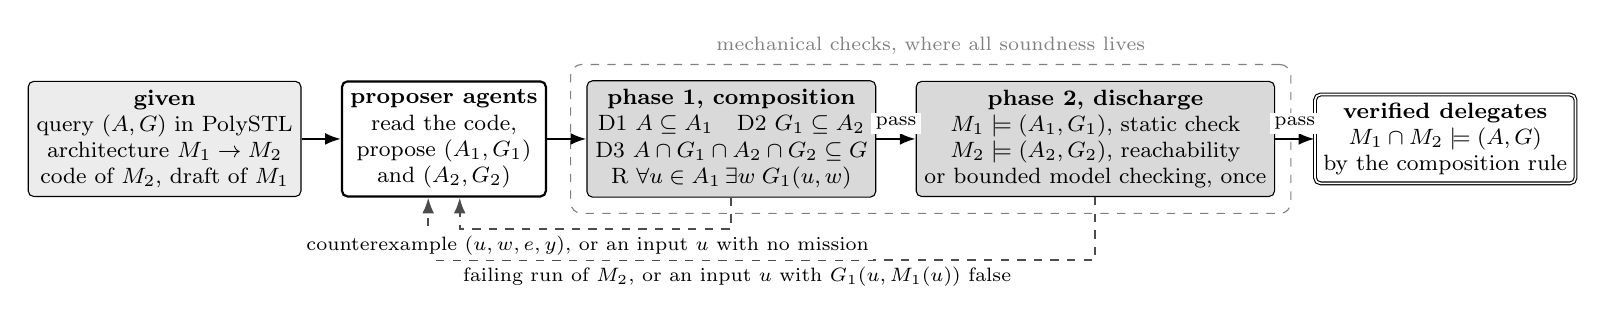
\begin{tikzpicture}[
  font=\footnotesize,
  box/.style={draw, rounded corners=2pt, align=center, inner sep=3pt, minimum height=8mm},
  given/.style={box, fill=gray!15},
  agent/.style={box, fill=white, thick},
  check/.style={box, fill=gray!30},
  result/.style={box, fill=white, double},
  arr/.style={-{Latex[length=2mm]}, thick},
  back/.style={-{Latex[length=2mm]}, thick, dashed, gray!60!black},
  lbl/.style={font=\scriptsize, align=center, fill=white, inner sep=1.5pt}
]
\node[given] (in) {\textbf{given}\\query $(A,G)$ in PolySTL\\architecture $M_1\to M_2$\\code of $M_2$, draft of $M_1$};
\node[agent, right=5mm of in] (prop) {\textbf{proposer agents}\\read the code,\\propose $(A_1,G_1)$\\and $(A_2,G_2)$};
\node[check, right=5mm of prop] (p1) {\textbf{phase 1, composition}\\D1 $A\subseteq A_1$\quad D2 $G_1\subseteq A_2$\\D3 $A\cap G_1\cap A_2\cap G_2\subseteq G$\\R $\forall u\in A_1\,\exists w\;G_1(u,w)$};
\node[check, right=5mm of p1] (p2) {\textbf{phase 2, discharge}\\$M_1\models(A_1,G_1)$, static check\\$M_2\models(A_2,G_2)$, reachability\\or bounded model checking, once};
\node[result, right=5mm of p2] (res) {\textbf{verified delegates}\\$M_1\cap M_2\models(A,G)$\\by the composition rule};
\draw[arr] (in) -- (prop);
\draw[arr] (prop) -- (p1);
\draw[arr] (p1) -- node[lbl, above=0.5mm] {pass} (p2);
\draw[arr] (p2) -- node[lbl, above=0.5mm] {pass} (res);
\coordinate (f1) at ($(p1.south)+(0,-4mm)$);
\coordinate (f2) at ($(p2.south)+(0,-8mm)$);
\draw[back] (p1.south) -- (f1) -| ($(prop.south)+(2mm,0)$);
\draw[back] (p2.south) -- (f2) -| ($(prop.south)+(-2mm,0)$);
\node[lbl, below=0.3mm] at ($(f1)!0.5!(f1 -| prop.south)$) {counterexample $(u,w,e,y)$, or an input $u$ with no mission};
\node[lbl, below=0.3mm] at ($(f2)!0.55!(f2 -| prop.south)$) {failing run of $M_2$, or an input $u$ with $G_1(u,M_1(u))$ false};
\begin{scope}[on background layer]
\node[draw, gray, dashed, rounded corners, fit=(p1) (p2), inner sep=2mm, label={[gray, font=\scriptsize]above:mechanical checks, where all soundness lives}] {};
\end{scope}
\end{tikzpicture}}
\caption{Agentic delegation. Proposer agents read the query, the architecture and the source code and propose candidate delegates; phase 1 checks the composition conditions and realizability on formulas alone; phase 2 discharges each component against its delegate, the planner by a static check and the controller once by reachability or bounded model checking; every failure returns a counterexample to the proposers, and a pair that passes both phases is sound regardless of how it was proposed.}
\label{fig:agentic}
\end{figure*}

\section{Text}
Filler text so the figure has somewhere to float. Figure~\ref{fig:agentic} shows the framework.
\end{document}
